%usepackage es egyebek
\input{./globdef}
\input{./tcboxdef}
% ez valahol kellett
\DeclarePairedDelimiter\ceil{\lceil}{\rceil}
\DeclarePairedDelimiter\floor{\lfloor}{\rfloor}

% zárójelek stb.
\newcommand{\Gzjel}[1]{%
{ \left( #1 \right) }
}

\newcommand{\gzjel}[1]{%
{ \left( #1 \right) }
}

\newcommand{\Toligv}[2]{%
#1,\hdots ,#2
}

\newcommand{\GZJ}[1]{%
{ \left( #1 \right) }
}

\newcommand{\KZJ}[1]{%
{ \{ #1 \} }
}

\newcommand{\szzjel}[1]{%
{ \left[ #1 \right] }
}

\newcommand{\Tolig}[2]{%
#1\hdots #2
}

\newcommand{\SZOR}[2]{%
#1\cdot\hdots\cdot #2
}

% integrál rendes d-vel
\newcommand{\mint}[2]{%
\int #1 \text{d}#2
}

% integrál rendes d-vel
\newcommand{\mhint}[4]{%
\int_{#1}^{#2} #3 \text{d}#4
}

\newcommand{\mhpfv}[3]{%
\left [ #3 \right ]_{ #1 }^{ #2 }
}

\newcommand{\mder}[2]{%
\frac{\text{d} #1}{\text{d}#2}
}


% ez máshogy van alapban
\newcommand{\tg}[0]{%
\tan
}

\newcommand{\ctg}[0]{%
\cot
}

\newcommand{\D}[1]{%
{{\mathbb{D}\szzjel{#1}}}
}

\newcommand{\V}[1]{%
{{{\mathbb{D}}^{2}\szzjel{#1}}}
}


\newcommand{\E}[1]{%
{{\mathbb{E}\szzjel{#1}}}
}

\newcommand{\A}[1]{%
{\mathbb{A}\szzjel{#1}}
}

\newcommand{\hehu}[1]{%
\hspace{0.5cm}#1\hspace{0.5cm}
}

\newcommand{\bmx}[1]{%
\begin{bmatrix}
#1
\end{bmatrix}
}

\newcommand{\mx}[1]{%
\begin{matrix}
#1
\end{matrix}
}

\newcommand{\gjmx}[2]{%
\left[
\begin{array}{@{}c|c@{}}
#1 & #2
\end{array}
\right]
}




\input{./szavakdef}
\input{./altalanos}


%\hyphenation{-transz-for-mált-ját}

\newcommand{\opover}[2]{%
\kh \overset{ #1 }{ #2 } \kh
}

\newcounter{szam}
\newcommand{\sectC}[1]{%
\stepcounter{szam}
\noindent {\bf \arabic{szam}. #1 }
}
\newcommand{\sect}[1]{%
\noindent {\newline \bf #1}
}

\newcommand{\myeq}[2]{%
\begin{equation*}
\label{eq:#1}\tag{#1}
#2
\end{equation*}
}

\newcommand{\gat}[1]{%
\begin{gather*}
#1
\end{gather*}
}

\begin{document}
\begin{spacing}{1.3}

\sect{Intuitív áttekintés}\newline
\begin{itemize}
   \item Euler azonosság:
   \myeq{Eulerid}{e^{it}=\cos(t)+i\sin(t) \ \ \ (t\in\mathbb{R})}

   \item $e^{i n \pi}=e^{-i n \pi}=(-1)^n\ \ \ n\text{ egész}$
   \item $\cos(t)=\frac{e^{it}+e^{-it}}{2}$
   \item $\sin(t)=\frac{e^{it}-e^{-it}}{2i}$
   \item komplex integrál valós intervallumon:
   \myeq{compint}{\mhint{a}{b}{A(t)+iB(t)}{t}=
   \mhint{a}{b}{A(t)}{t}+i\mhint{a}{b}{B(t)}{t}}
   \item 
      \myeq{trigint}{
      \mhint{-\pi}{\pi}{e^{int}}{t}=
         \begin{cases}
         0&\ \ \ n\neq 0\ \ n\text{ egész}\\
         2\pi \ \ n=0
         \end{cases} 
      }
\item Dirichlet feltételek: \href{https://en.wikipedia.org/wiki/Dirichlet_conditions}{wiki}\\
\end{itemize}

\vspace{0.5cm}
\sect{Együtthatók}
Legyen $f$ egy $2\pi$ periodikus valós függvény, keressük a 
$c_n\in \mathbb{C}$ számokat, melyekkel
\gat{
f(t)=\sum_{n=-\infty}^{\infty} c_{n} e^{int}}

$e^{-imt}$-vel szorozva és integrálva:

\gat{
c_{m}=\frac{1}{2\pi}\mhint{-\pi}{\pi}{f(t)e^{-imt}}{t} \ \ \ (m\in \mathbb{Z})}
Klasszikus alak:
\gat{
f(t)=c_{0}+\sum_{n=1}^{\infty} a_{n} \cos(nt) + \sum_{n=1}^{\infty} b_{n} \sin(nt)}

Összevetve $m>0$-ra:
\gat{
\frac{1}{2}\left( a_m + \frac{b_m}{i} \right) = c_{m}  \\
\frac{1}{2}\left( a_m - \frac{b_m}{i} \right) = c_{-m} \\
a_{m}=c_{m}+c_{-m}=\frac{1}{\pi}\mhint{-\pi}{\pi}{f(t)\cos(mt)}{t}\\
b_{m}=i(c_{m}-c_{-m})=\frac{1}{\pi}\mhint{-\pi}{\pi}{f(t)\sin(mt)}{t}
}

\sect{Tulajdonságok:}
\begin{itemize}
\item $c_{m}$ és $c_{-m}$ konjugáltak
\item Ha $f$ páros, akkor $b_{m}=0$
\item Ha $f$ páratlan, akkor $a_{m}=0$
\item $e_{m}(t)=e^{imt}$ jelöléssel és 
a $(a,b)=\frac{\mhint{-\pi}{\pi}{a(t)\overline{b(t)}}{t}}{2\pi}$ belső szorzattal az $f$ $FS$-ának  
együtthatói az $\{ e_m \} $ ortonormált rendszerbeli kooridináták:
\begin{equation*}
   f=\sum_{n=-\infty}^{\infty} (f,e_{n})e_{n}=\sum_{n=-\infty}^{\infty} c_{n}e_{n}
\end{equation*}

\item érvényes a Parseval azonosság:
\myeq{Parsevalid}{
   \frac{1}{2\pi}\mhint{-\pi}{\pi}{|f(t)|^2}{t} = \sum_{n=-\infty}^{\infty} |c_{n}|^2 =
   c_{0}^2 + \frac{1}{2}\sum_{n=1}^{\infty} \left( a_{n}^2+b_{n}^2 \right)
}
\end{itemize}


%\end{spacing}
\sect{Jelölés: }
$FS$ = Fourier-sor\\

\sect{Megjegyzés} Egy véges intervallumon definiált függvény esetén 
az $\mathbb{R}$-re való periodikus kiterjesztésére gondolunk.

\sect{Feladatok}\newline

\sectC{Feladat} Számoljuk ki a következő \fv{}$FS$-át:
\myeq{negyszog}{
f(t) =
   \begin{cases*}
      -1 & $-\pi \le t < 0$\\
      0  & t=0\\
      1  & $ 0 < t \le \pi$
   \end{cases*}
}

\sect{Megoldás}
$f$ páratlan, így $c_{0}=a_{m}=0$. 
\gat{
b_m=\frac{1}{\pi}\mhint{-\pi}{\pi}{f(t)\sin(mt)}{t}=\\
\frac{2}{\pi}\mhint{0}{\pi}{\sin(mt)}{t}=
\frac{2}{\pi}\left( \frac{-\cos(m\pi)}{m}-\frac{-\cos(m0)}{m}\right)=\\
=\frac{2}{m\pi}\left( 1-(-1)^{m}\right) \\
}
Ha $m$ páros $b_{m}=0$.
\gat{
b_{2m-1}=\frac{4}{(2m-1)\pi}\\
f(t)=\sum_{n=1}^{\infty} \frac{4}{(2n-1)\pi}\sin((2n-1)t)=
\frac{4}{\pi}\sum_{n=1}^{\infty} \frac{\sin((2n-1)t)}{2n-1}
}

\sectC{Feladat} Ábrázoljuk a \eqref{eq:negyszog} \fv{t} és $FS$-ának részletösszegét néhány tagig.\\
\sect{Megoldás} 
\href{M/negyszog.m}{negyszog.m}
\begin{center}
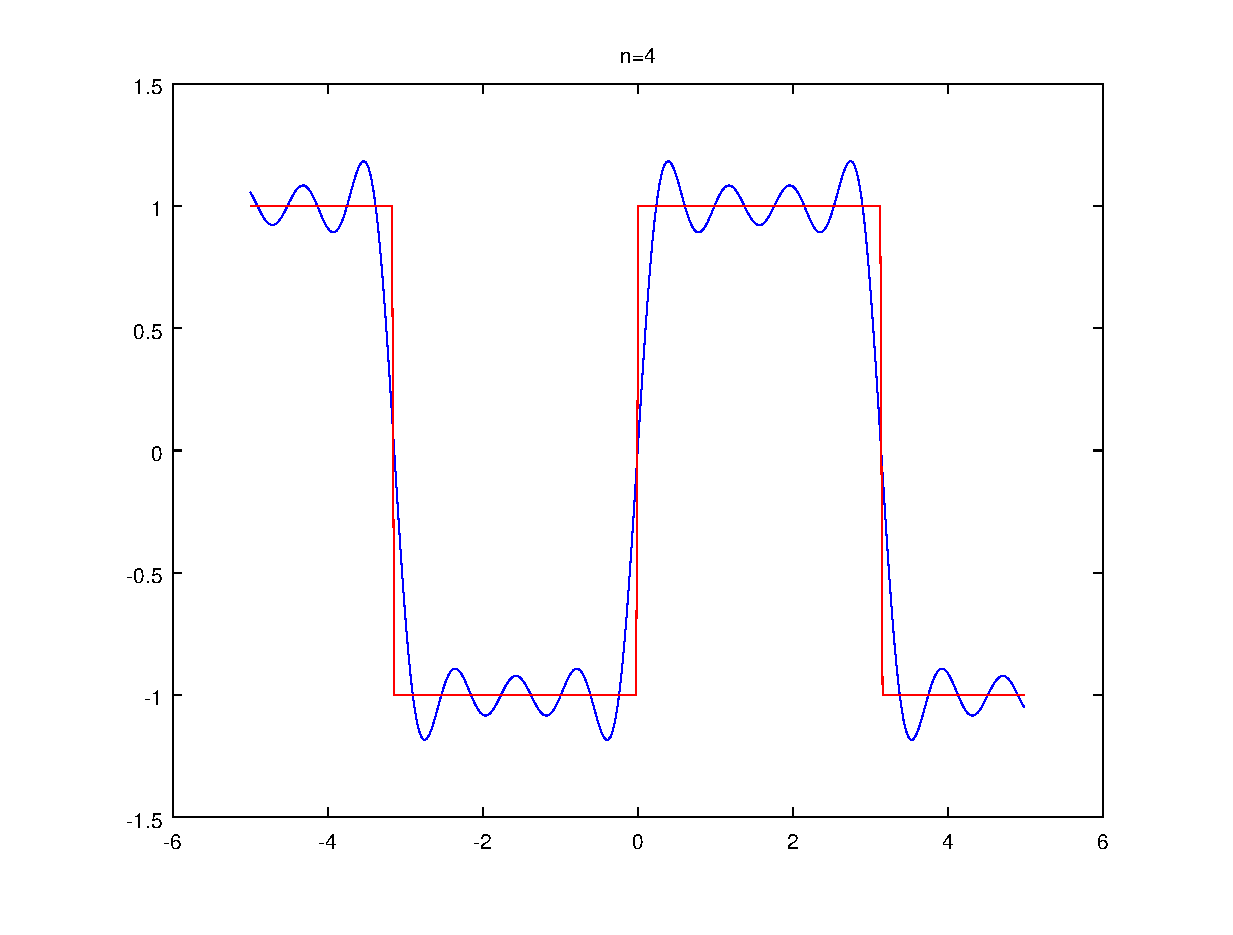
\includegraphics[width=20cm,height=10.1cm]{M/negyszog.eps}
%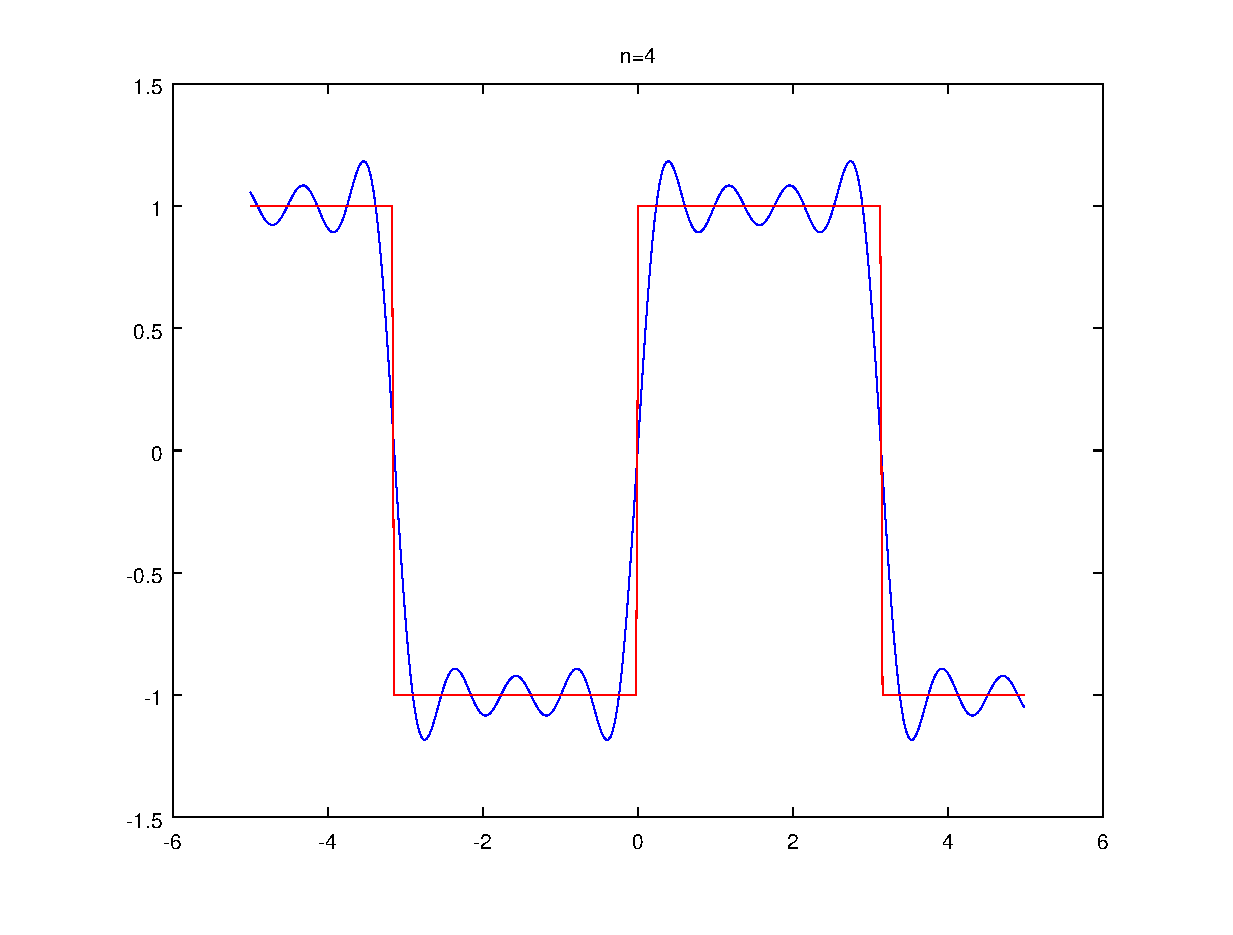
\includegraphics[scale=1]{M/negyszog.eps}
\end{center}


\sectC{Feladat } Milyen kapcsolat van a \eqref{eq:negyszog} és $g$ között? 
\gat{
g(t) =
   \begin{cases}
      a & A \le t < \frac{A+B}{2}\\
      \frac{a+b}{2}  & t=\frac{A+B}{2}\\
      b  & \frac{A+B}{2} < t \le B
   \end{cases}
}
adott $a<b,\ A<B$ valósak esetén.
\newline\sect{Megoldás} Az $[A,B]$ intervallum $[-\pi,\pi]$-be "vihető" 
a $\varphi(t)=-\pi+\frac{2\pi}{B-A}(t-A)$ belső transzformációval. Az $f(\varphi(t))$ 
már jó helyen van. Az értékeit a $\phi(t)=\frac{b-a}{2}t+\frac{a+b}{2}$ átalakítással 
állítjuk be. Tehát $g(t)=\phi(f(\varphi(t)))$.

\vspace{0.5cm}
\sectC{Példa }  
\myeq{transz}{
g(t) =
   \begin{cases}
      1 & 2 \le t < 5\\
      3 & t=5\\
      5  & 5 < t \le 8
   \end{cases}
}
esetén a $FS$:
\gat{
3+\frac{8}{\pi}\sum_{n=1}^{\infty} \frac{\sin((2n-1)\left(\frac{2\pi}{3}t-\pi\right))}{(2n-1)}
}

\sect{Megjegyzés} Ez utóbbi összeg nem $FS$ a definíció szerint.
\newline
\sectC{Feladat} Győződjünk meg program segítségével a \eqref{eq:transz}-beli átalakítás 
helyességéről.
\sect{Megoldás} A \eqref{eq:negyszog}-nél használt programot átalakítva:
\href{M/transz.m}{transz.m}
%~ \begin{center}
%~ 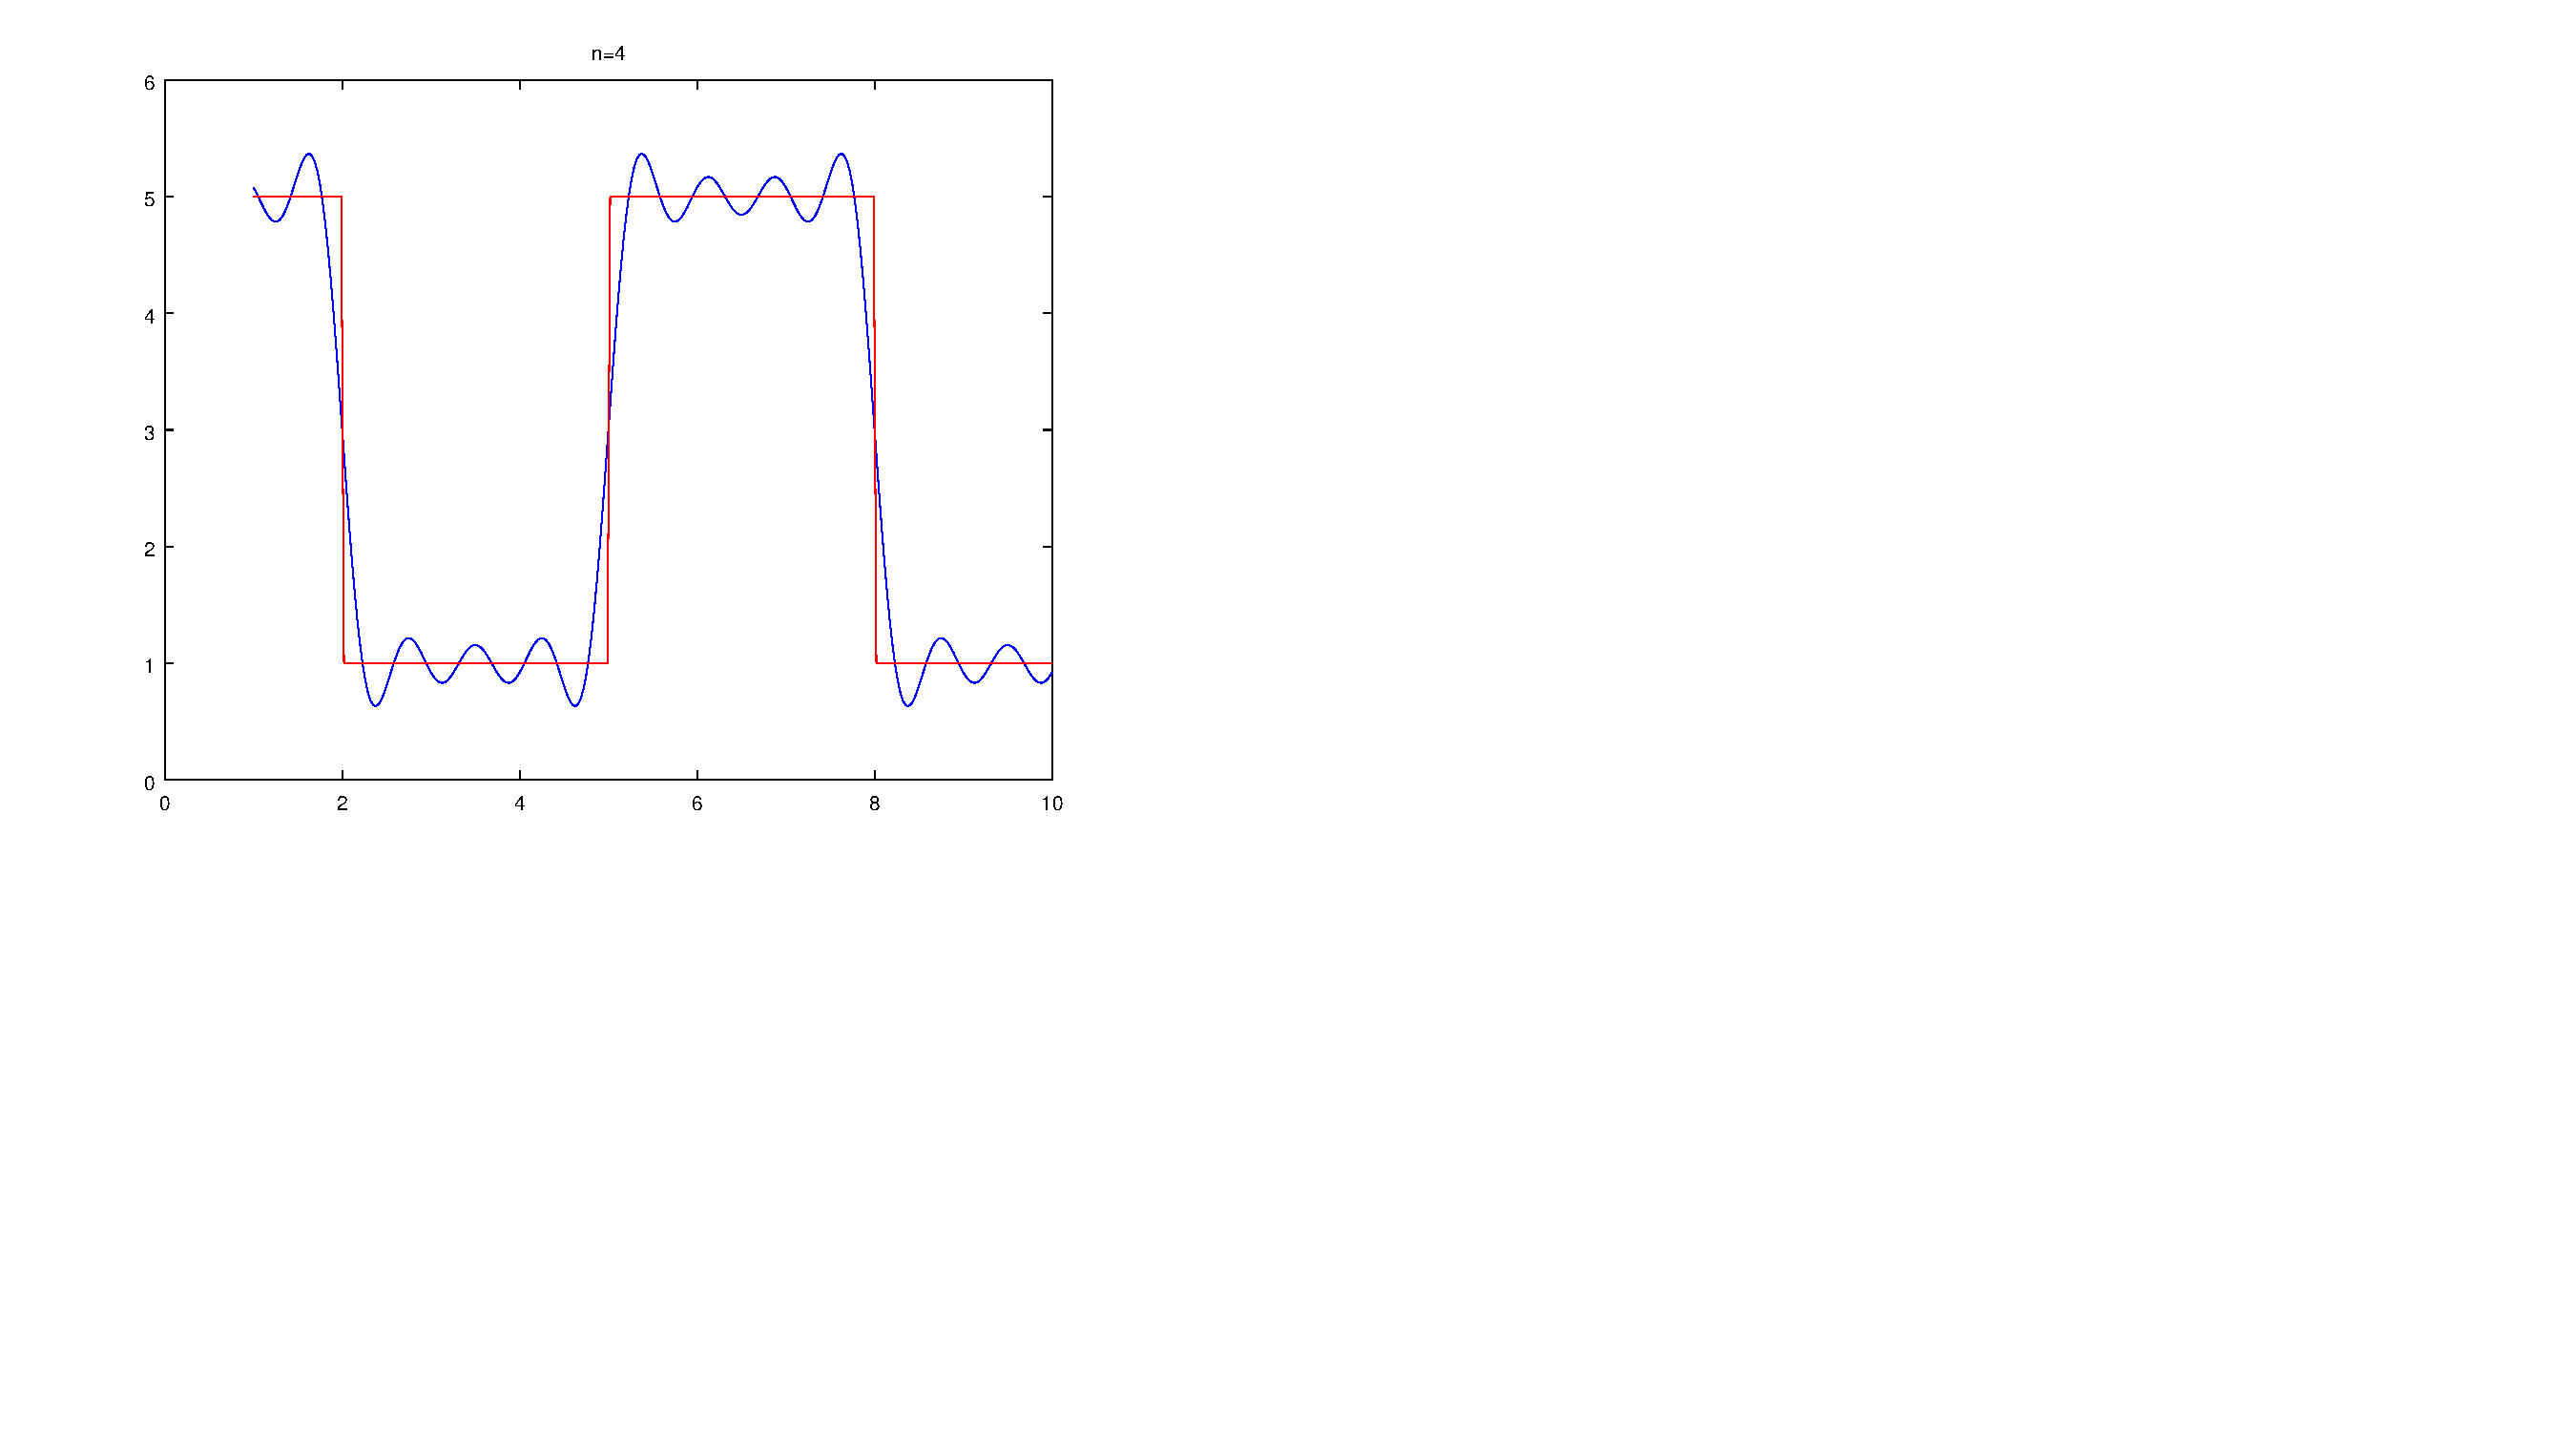
\includegraphics[width=24cm,height=12.1cm]{M/transz.eps}
%~ \end{center}



\sectC{Feladat} Mutassuk meg, hogy 
\gat{
\sum_{n=1}^{\infty}\frac{(-1)^{n+1}}{(2n-1)}=\frac{\pi}{4}
}
\sect{Megoldás} Induljunk ki a $f(\frac{\pi}{2})=1$-ből ($f$ a \eqref{eq:negyszog}-beli). 


\vspace{0.2cm}
\sectC{Feladat} Számoljuk ki a következő \fv{}$FS$-át:
\myeq{saw}{
f(t) = t,\ \ \ t\in [-\pi,\pi] 
}
\sect{Megoldás }
$f$ páratlan, így $c_{0}=a_{m}=0$. 
\gat{
\pi b_m=\mhint{-\pi}{\pi}{t\sin(mt)}{t}=\\
\frac{\pi(-\cos(m\pi))-(-\pi)(-\cos(-m\pi))}{m}-\mhint{-\pi}{\pi}{\frac{-\cos(mt)}{m}}{t}=
\frac{2\pi(-1)^m}{m}-0\\
f(t)=2\sum_{n=1}^{\infty} \frac{(-1)^{m+1} \sin(mt)}{m}
}


\sectC{Feladat} Ábrázoljuk a \eqref{eq:saw} \fv{t} és $FS$-ának részletösszegét néhány tagig.\\
\sect{Megoldás} 
\href{M/saw.m}{saw.m}
\begin{center}
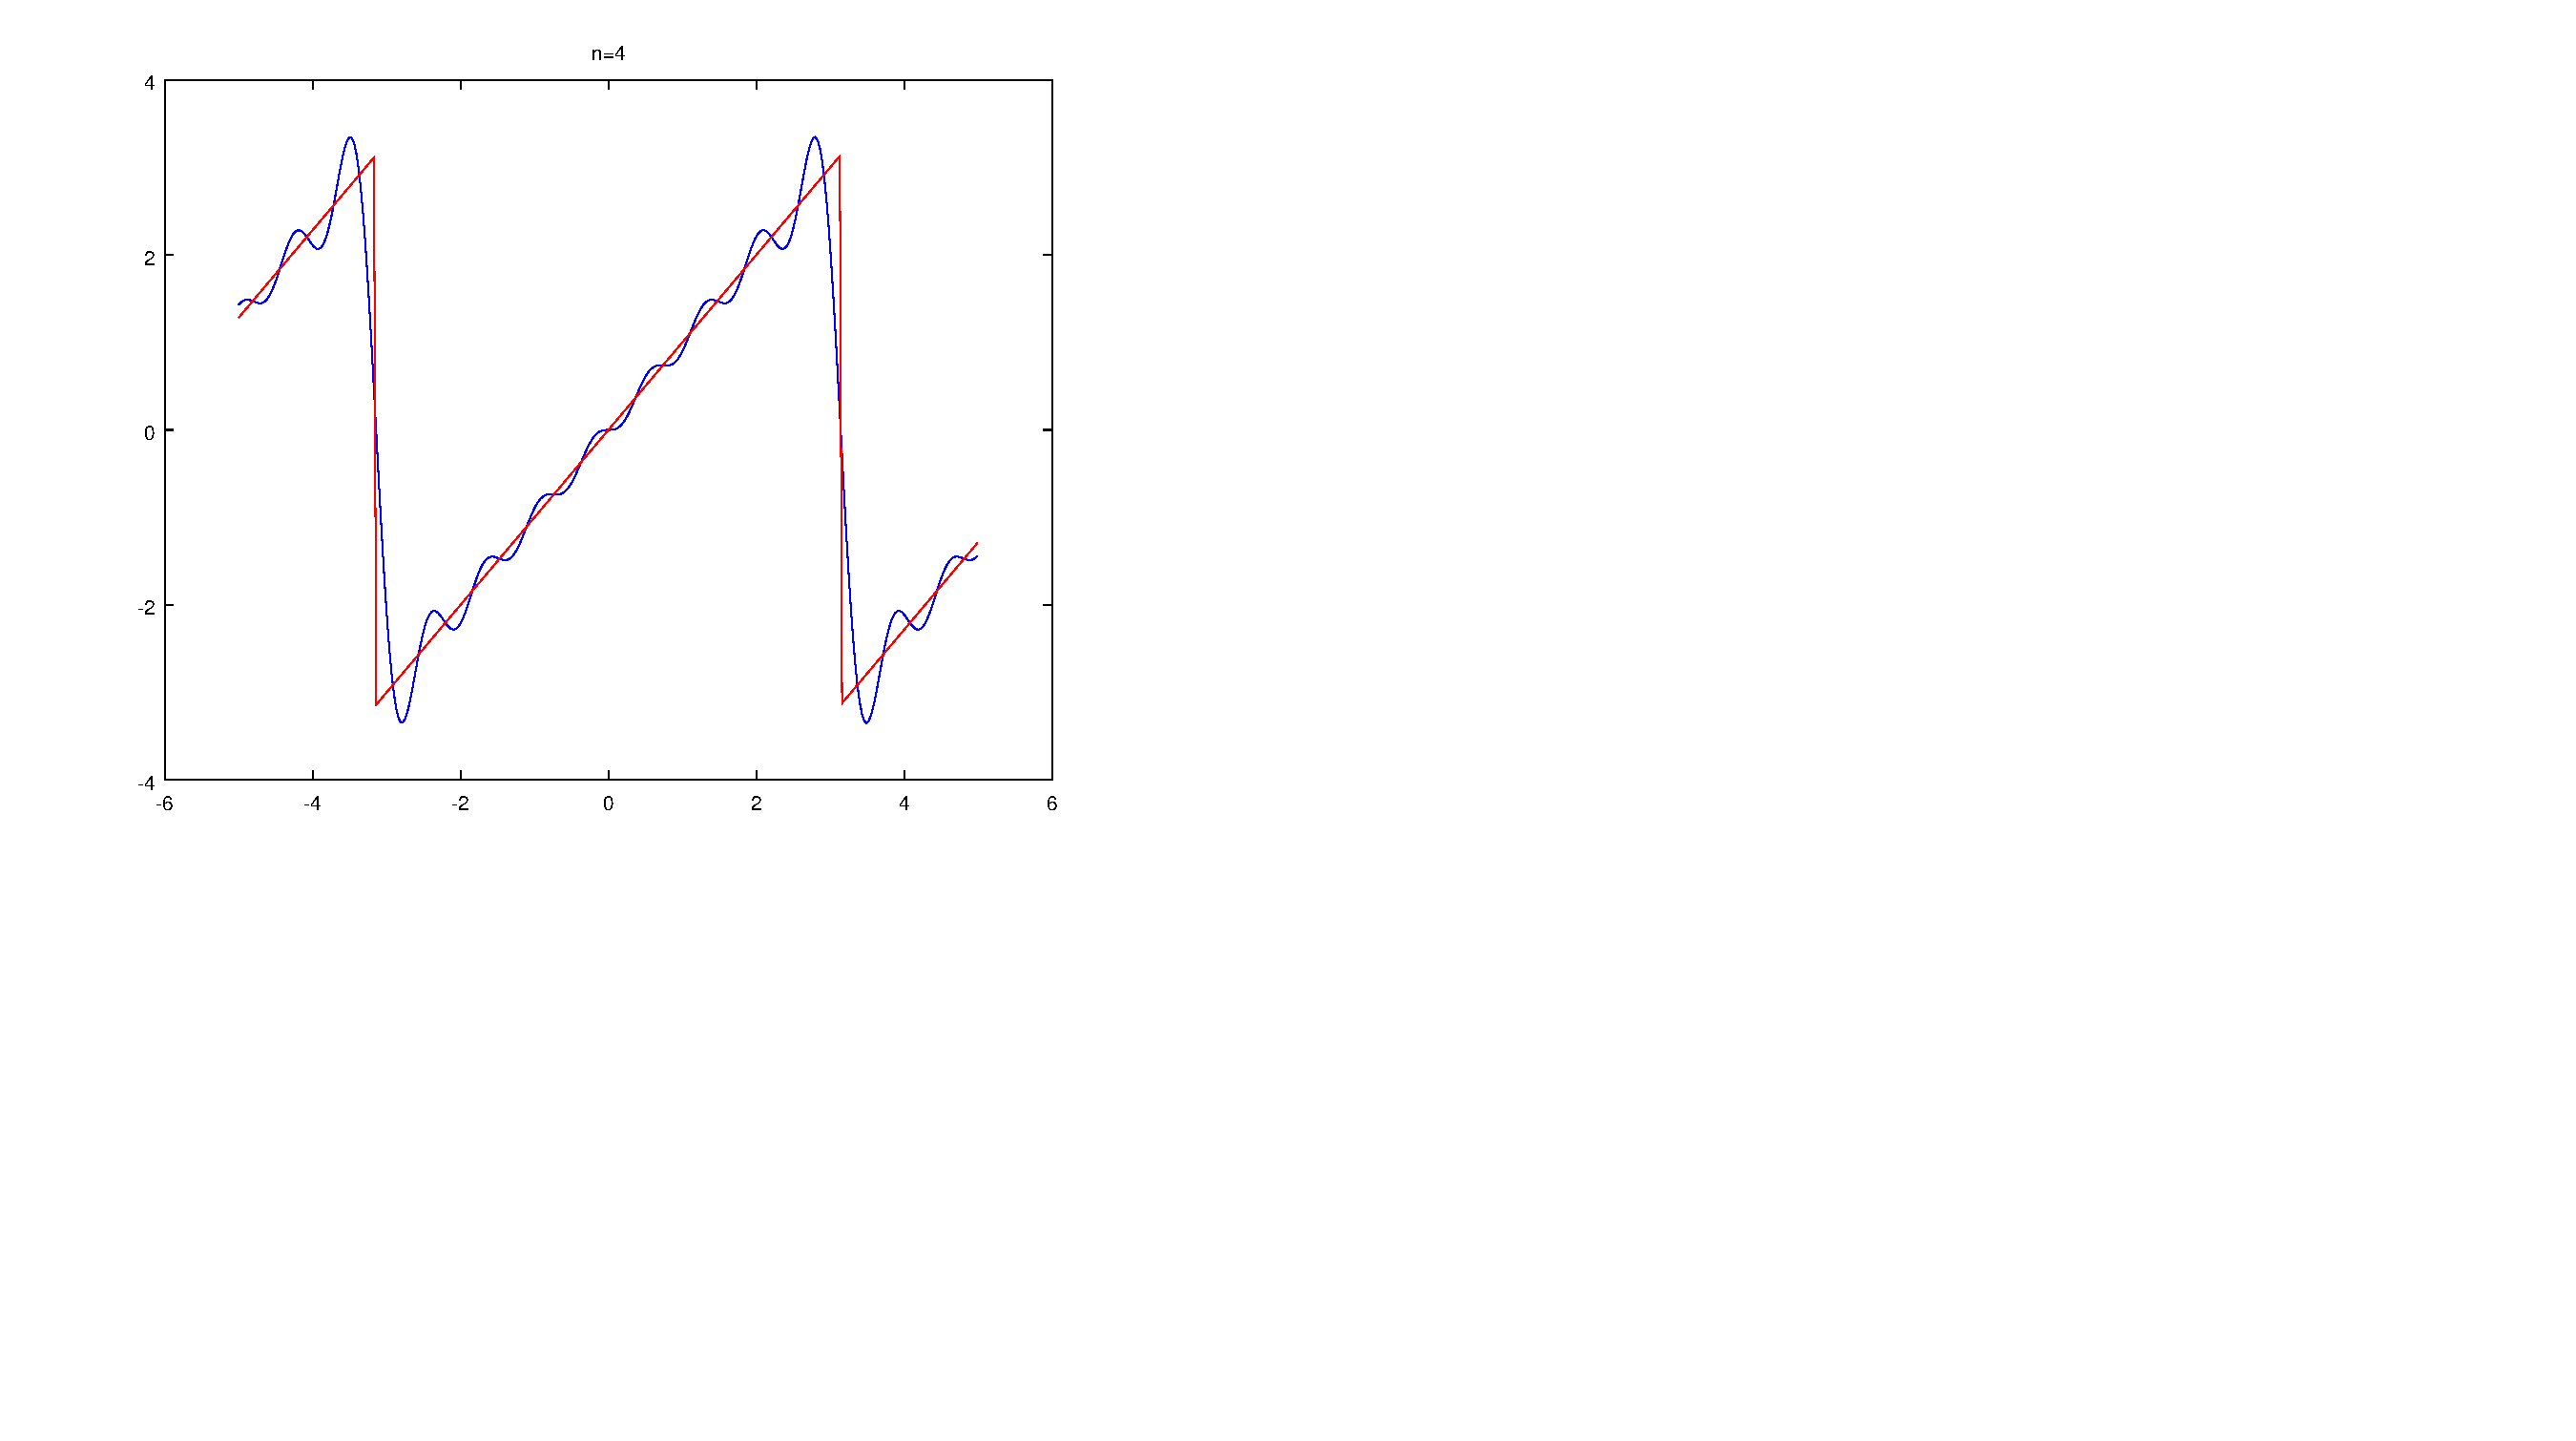
\includegraphics[width=44cm,height=12.1cm]{M/saw.eps}
\end{center}

\sectC{Feladat} Mutassuk meg, hogy 
\myeq{recn2}{
\sum_{n=1}^{\infty} \frac{1}{n^2}=\frac{\pi^2}{6}
}
\sect{Megoldás} Írjuk fel a \eqref{eq:saw}-ra a \eqref{eq:Parsevalid}-et:
\gat{
   \frac{1}{2\pi}\mhint{-\pi}{\pi}{|f(t)|^2}{t}=\frac{1}{2\pi} \left( \frac{\pi^3}{3}-\frac{(-\pi)^3}{3} \right)=\frac{\pi^2}{3}\\
   \sum_{n=-\infty}^{\infty} |c_{n}|^2=\frac{1}{2}\sum_{n=1}^{\infty} \frac{4}{n^2}
}


\vspace{0.2cm}
\sectC{Feladat} Számoljuk ki a következő \fv{}$FS$-át:
\myeq{absz}{
f(t) = \vert t\vert,\ \ \ t\in [-\pi,\pi] 
}
\sect{Megoldás }
$f$ páros, így $b_{m}=0$. 
\gat{
2\pi c_{0}=\mhint{-\pi}{\pi}{\vert t\vert}{t}=\pi^2\ \ \ c_{0}=\frac{\pi}{2}\\
\pi a_m=2\mhint{0}{\pi}{t\cos(mt)}{t}=0-2\mhint{0}{\pi}{\frac{\sin(mt)}{m}}{t}=\\
=\frac{2}{m^2}\left( \cos(m\pi)-\cos(m0)  \right)=\frac{2}{m^2}\left( (-1)^{m}-1  \right)\\
a_{2m-1}=-\frac{4}{(2m-1)^2}\\
f(t)=\frac{\pi}{2}-\frac{4}{\pi}\sum_{n=1}^{\infty}\frac{\cos((2m-1)t)}{(2m-1)^2}
}

\sectC{Feladat} Ábrázoljuk a \eqref{eq:absz} \fv{t} és $FS$-ának részletösszegét néhány tagig.\\
\sect{Megoldás} 
\href{M/absz.m}{absz.m}
\begin{center}
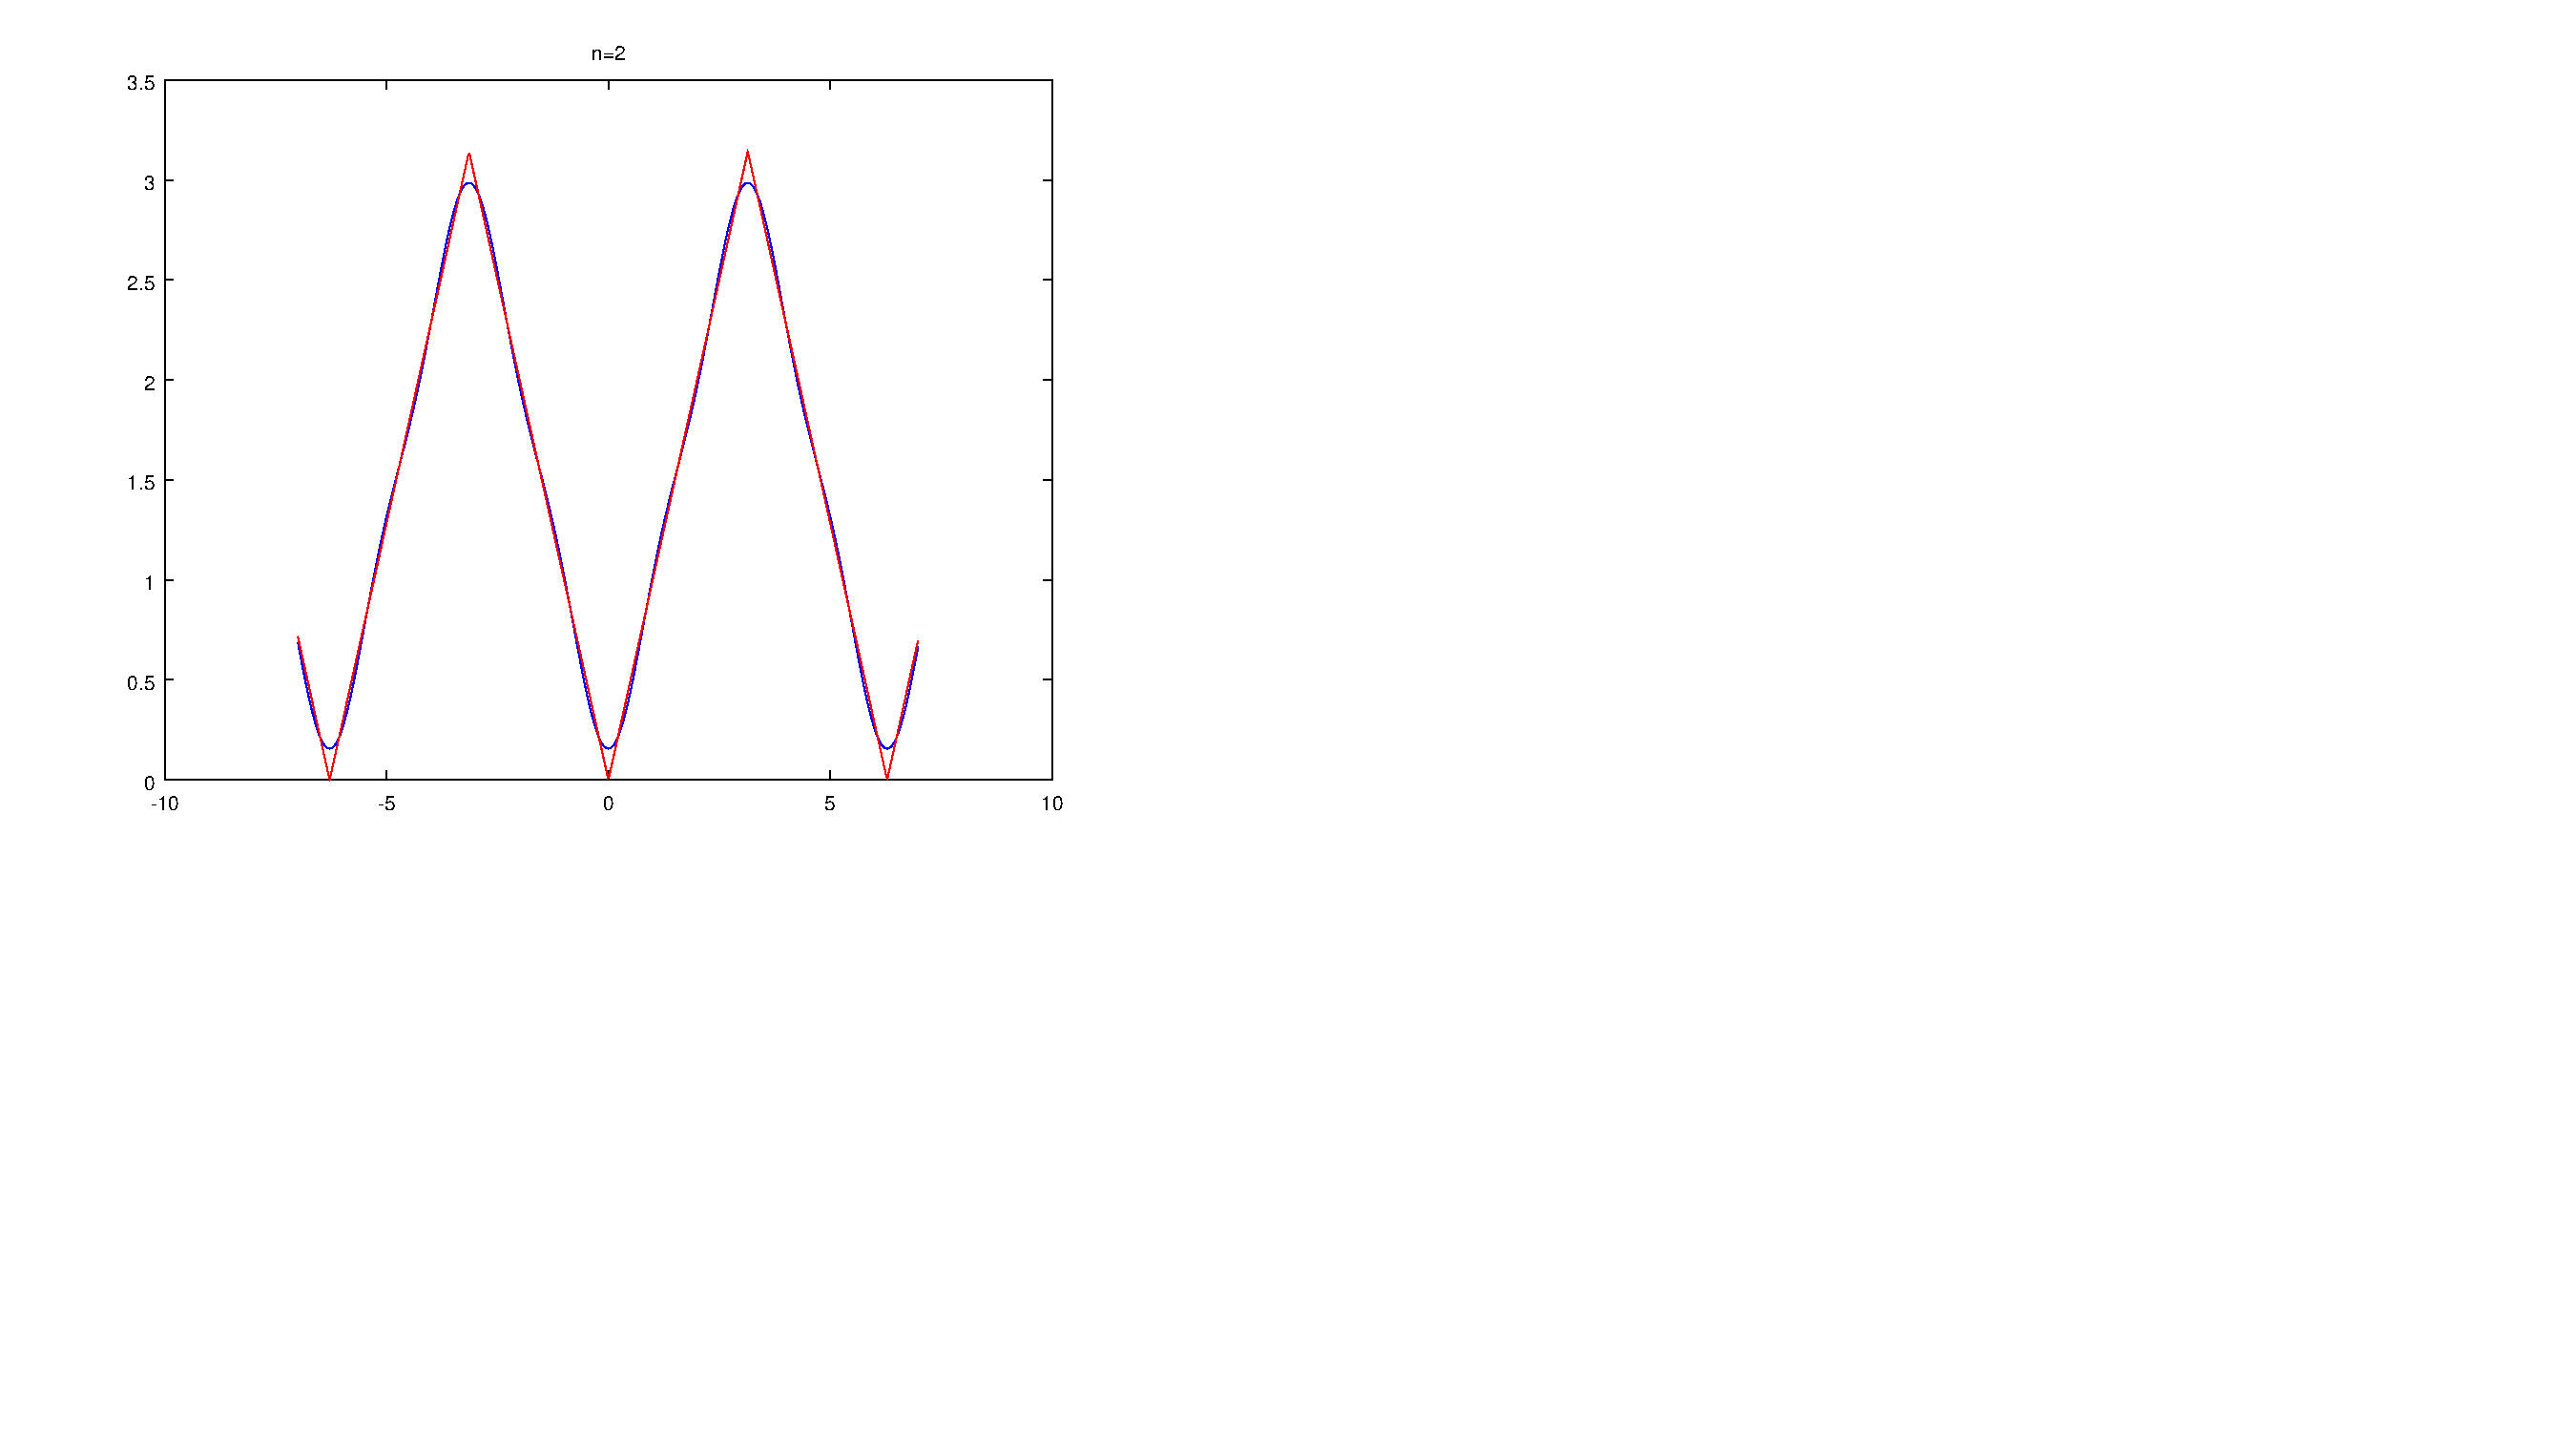
\includegraphics[width=40cm,height=8.1cm]{M/absz.eps}
\end{center}



\end{spacing}
\end{document}
